\documentclass[preview]{standalone}
\usepackage{geometry}

%graphics

\usepackage{tikz}
\usetikzlibrary{shapes.geometric, shapes.multipart, arrows, calc, through,intersections,circuits.logic.US}
\usepackage[caption=false,font=footnotesize]{subfig}

\tikzset{
    pics/vcell/.style = {
        code = {%
        \coordinate (-center) at (0, 0);
        \coordinate (-north) at (0, .5cm);
        \coordinate (-south) at (0,-.5cm);
        \coordinate (-se) at (310:.5cm);
        \coordinate (-sw) at (230:.5cm);
        \coordinate (-ne) at (50:.5cm);
        \coordinate (-nw) at (130:.5cm);
        \draw[line width=1pt](0,0)circle[radius=.5cm];
        }
    },
}
\begin{document}
\begin{figure}[!t]
\centering
\subfloat[]{
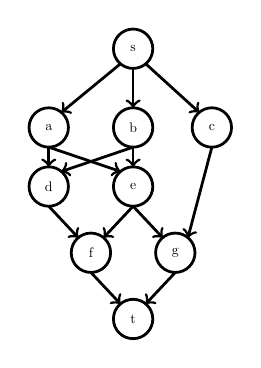
\begin{tikzpicture}[scale=0.5,transform shape, line width=1pt]
\pic(t) at (0,0) {vcell};
\node at (t-center) {t};

\pic(f) at ($(t-nw)+(120:1.5cm)$){vcell};
\node at (f-center) {f};
\draw[->] (f-south) -- (t-nw);

\pic(g) at ($(t-ne)+(60:1.5cm)$){vcell};
\node at (g-center) {g};
\draw[->] (g-south) -- (t-ne);

\pic(d) at ($(f-nw)+(120:1.5cm)$){vcell};
\node at (d-center) {d};
\draw[->] (d-south) -- (f-nw);

\pic(e) at ($(f-ne)+(60:1.5cm)$){vcell};
\node at (e-center) {e};
\draw[->] (e-south) -- (f-ne);
\draw[->] (e-south) -- (g-nw);

\pic(a) at ($(d-north)+(0,1cm)$){vcell};
\node at (a-center) {a};
\draw[->] (a-south) -- (d-north);
\draw[->] (a-south) -- (e-nw);

\pic(b) at ($(e-north)+(0,1cm)$){vcell};
\node at (b-center) {b};
\draw[->] (b-south) -- (e-north);
\draw[->] (b-south) -- (d-ne);

\pic(c) at ($(b-center)+(2,0)$){vcell};
\node at (c-center) {c};
\draw[->] (c-south) -- (g-ne);

\pic(s) at ($(b-north)+(0,1.5cm)$){vcell};
\node at (s-center) {s};
\draw[->] (s-south) -- (b-north);
\draw[->] (s-sw) -- (a-ne);
\draw[->] (s-se) -- (c-nw);
\end{tikzpicture}
}
\subfloat[]{
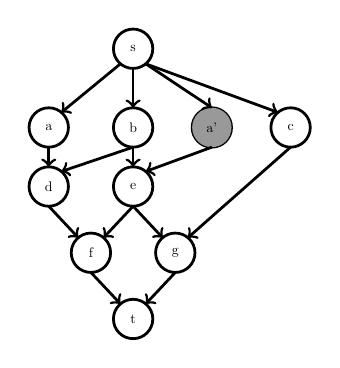
\begin{tikzpicture}[scale=0.5,transform shape, line width=1pt]
\pic(t) at (0,0) {vcell};
\node at (t-center) {t};

\pic(f) at ($(t-nw)+(120:1.5cm)$){vcell};
\node at (f-center) {f};
\draw[->] (f-south) -- (t-nw);

\pic(g) at ($(t-ne)+(60:1.5cm)$){vcell};
\node at (g-center) {g};
\draw[->] (g-south) -- (t-ne);

\pic(d) at ($(f-nw)+(120:1.5cm)$){vcell};
\node at (d-center) {d};
\draw[->] (d-south) -- (f-nw);

\pic(e) at ($(f-ne)+(60:1.5cm)$){vcell};
\node at (e-center) {e};
\draw[->] (e-south) -- (f-ne);
\draw[->] (e-south) -- (g-nw);

\pic(a) at ($(d-north)+(0,1cm)$){vcell};
\node at (a-center) {a};
\draw[->] (a-south) -- (d-north);

\pic(b) at ($(e-north)+(0,1cm)$){vcell};
\node at (b-center) {b};
\draw[->] (b-south) -- (e-north);
\draw[->] (b-south) -- (d-ne);

\pic(aa) at ($(b-center)+(2,0)$){vcell};
\fill[color=gray!80] (aa-center) circle[radius=.5];
\node at (aa-center) {a'};
\draw[->] (aa-south) -- (e-ne);

\pic(c) at ($(aa-center)+(2,0)$){vcell};
\node at (c-center) {c};
\draw[->] (c-south) -- (g-ne);

\pic(s) at ($(b-north)+(0,1.5cm)$){vcell};
\node at (s-center) {s};
\draw[->] (s-south) -- (b-north);
\draw[->] (s-sw) -- (a-ne);
\draw[->] (s-se) -- (c-nw);
\draw[->] (s-se) -- (aa-north);
\end{tikzpicture}
}
\subfloat[]{
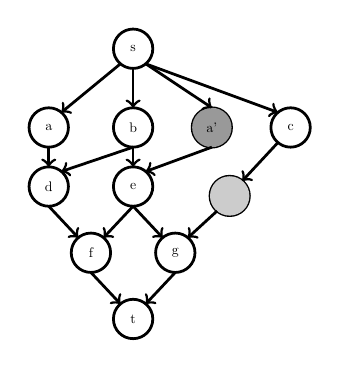
\begin{tikzpicture}[scale=0.5,transform shape, line width=1pt]
\pic(t) at (0,0) {vcell};
\node at (t-center) {t};

\pic(f) at ($(t-nw)+(120:1.5cm)$){vcell};
\node at (f-center) {f};
\draw[->] (f-south) -- (t-nw);

\pic(g) at ($(t-ne)+(60:1.5cm)$){vcell};
\node at (g-center) {g};
\draw[->] (g-south) -- (t-ne);

\pic(d) at ($(f-nw)+(120:1.5cm)$){vcell};
\node at (d-center) {d};
\draw[->] (d-south) -- (f-nw);

\pic(e) at ($(f-ne)+(60:1.5cm)$){vcell};
\node at (e-center) {e};
\draw[->] (e-south) -- (f-ne);
\draw[->] (e-south) -- (g-nw);

\pic(w) at ($(g-ne)+(45:1.5cm)$){vcell};
\fill[color=gray!40] (w-center) circle[radius=.5cm];
\draw[->] (w-sw)--(g-ne);

\pic(a) at ($(d-north)+(0,1cm)$){vcell};
\node at (a-center) {a};
\draw[->] (a-south) -- (d-north);

\pic(b) at ($(e-north)+(0,1cm)$){vcell};
\node at (b-center) {b};
\draw[->] (b-south) -- (e-north);
\draw[->] (b-south) -- (d-ne);

\pic(aa) at ($(b-center)+(2,0)$){vcell};
\fill[color=gray!80] (aa-center) circle[radius=.5];
\node at (aa-center) {a'};
\draw[->] (aa-south) -- (e-ne);

\pic(c) at ($(aa-center)+(2,0)$){vcell};
\node at (c-center) {c};
\draw[->] (c-sw) -- (w-ne);

\pic(s) at ($(b-north)+(0,1.5cm)$){vcell};
\node at (s-center) {s};
\draw[->] (s-south) -- (b-north);
\draw[->] (s-sw) -- (a-ne);
\draw[->] (s-se) -- (c-nw);
\draw[->] (s-se) -- (aa-north);
\end{tikzpicture}
}
\end{figure}
\end{document}
